\documentclass[conference]{IEEEtran}
\usepackage{cite}
\usepackage{graphicx}
\usepackage{placeins}
\usepackage{caption}
\usepackage{subfigure}
\usepackage{enumerate}
\usepackage{afterpage}
\usepackage[font={small}]{caption}
\AtBeginDocument{\renewcommand{\abstractname}{Resumo}}
\begin{document}
\title{Projeto 1 de Introdu\c{c}\~ao ao Processamento de Imagens \\ Sexta Parte}
\author{\IEEEauthorblockN{Gabriel Martins de Miranda}
\IEEEauthorblockA{130111350\\
Universidade de Bras\'ilia\\
Email:gabrielmirandat@hotmail.com}
}
\maketitle
\begin{abstract}
O presente experimento realiza segmenta\c{c}\~ao da imagem building\_original, que no caso significa detec\c{c}\~ao de bordas, utilizando o algoritmo de Marr-Hildreth.
\end{abstract}

\section{ Introdu\c{c}\~ao} 
\label{sec:meth} 
	O detector de  Marr-Hildreth \'e conhecido por $Laplaciano $ $da $ $Gaussiana $, ou $LoG$, j\'a que consiste no uso do filtro que \'e a segunda derivada da gaussiana. O algoritmo consiste em:
\begin{itemize}
	\item Convoluir uma imagem de entrada f(x,y) com o filtro LoG.
	\item Encontrar o cruzamento por zero da imagem resultante, que consiste em substituir um pixel dela por ZERO caso em qualquer um das 3 dire\c{c}\~oes de um filtro 3x3 os pixels extremos possu\'irem sinais opostos.  
\end{itemize}
 
\section{Metodologia} 
\label{sec:meth} 
Para resolu\c{c}\~ao do problema seguiu$-$se os seguintes passos:

\begin{itemize}
	\item A convolu\c{c}\~ao de uma imagem pelo filtro LoG pode ser feita em duas etapas atrav\'es de manipula\c{c}\~ao alg\'ebrica. Pode-se primeiro convoluir a imagem pelo filtro gaussiano, criado utilizando-se a fun\c{c}\~ao $ fspecial( 'gaussian',25,4)$ , cujos par\^ametros indicam que usou-se um filtro de tamanho 25x25 e $\sigma$ = 4. Os valores da matriz resultante, ap\'os a convolu\c{c}\~ao,  se distribu\'iram em torno de 0.0000 e 0.0100, e ela foi chamada de $Ig$.
	\item Ap\'os calcula-se o laplaciano da imagem que resultou da etapa anterior, utilizando-se o filtro $hl = [1 1 1;1 -8 1; 1 1 1]$. A imagem resultante foi chamada $Ilog$.
	\item $Ilog$ foi convertida para uma imagem de sinais, valorada apenas com -1's, 0's e 1's. Para isto usou-se a fun\c{c}\~ao $sign$. O resultado foi armazenado em $sinais$.
	\item Faz-se a correla\c{c}\~ao de cada possibilidade de cruzamento por zero na imagem e armazena em cada passada em 4 imagens. A matriz que tem todas as transi\c{c}\~oes por zero foi chamada $y$.
	\item A imagem Log foi mascarada pelo cruzamento em zero, armazenando o resultado em $IlogM$.
	\item Atrav\'es do limiar de ZERO, criou-se uma imagem bin\'aria chamada $final$, composta pelos pixels $255$ caso $IlogM(i,j)>0$ ou pixels $0$ caso $IlogM(i,j)<0$.
	\item Em $final $ pode-se perceber o efeito espaguete que ocorre com este algoritmo. A etapa final consiste em remover este ru\'ido (efeito). Para isto, foi utilizado o mesmo processo de $final$, por\'em o limiar utilizado foi $2\%$ do valor m\'aximo da $Ilog$,(o livro prop\^os usar $4\%$, mas por observa\c{c}\~ao preferiu-se usar os  $2\%$), e ap\'os retirou-se todas as componentes menores de 7 pixels atrav\'es da fun\c{c}\~ao $bwareaopen(final2, 7)$. O resultado foi chamado$final2$.



\end{itemize}

\section{Resultados} 
\label{sec:meth} 
Resultados previstos na $Metodologia$:

		\vspace{2\baselineskip}\vspace{-\parskip}
		\begin{minipage}{\linewidth}
  		\centering
  		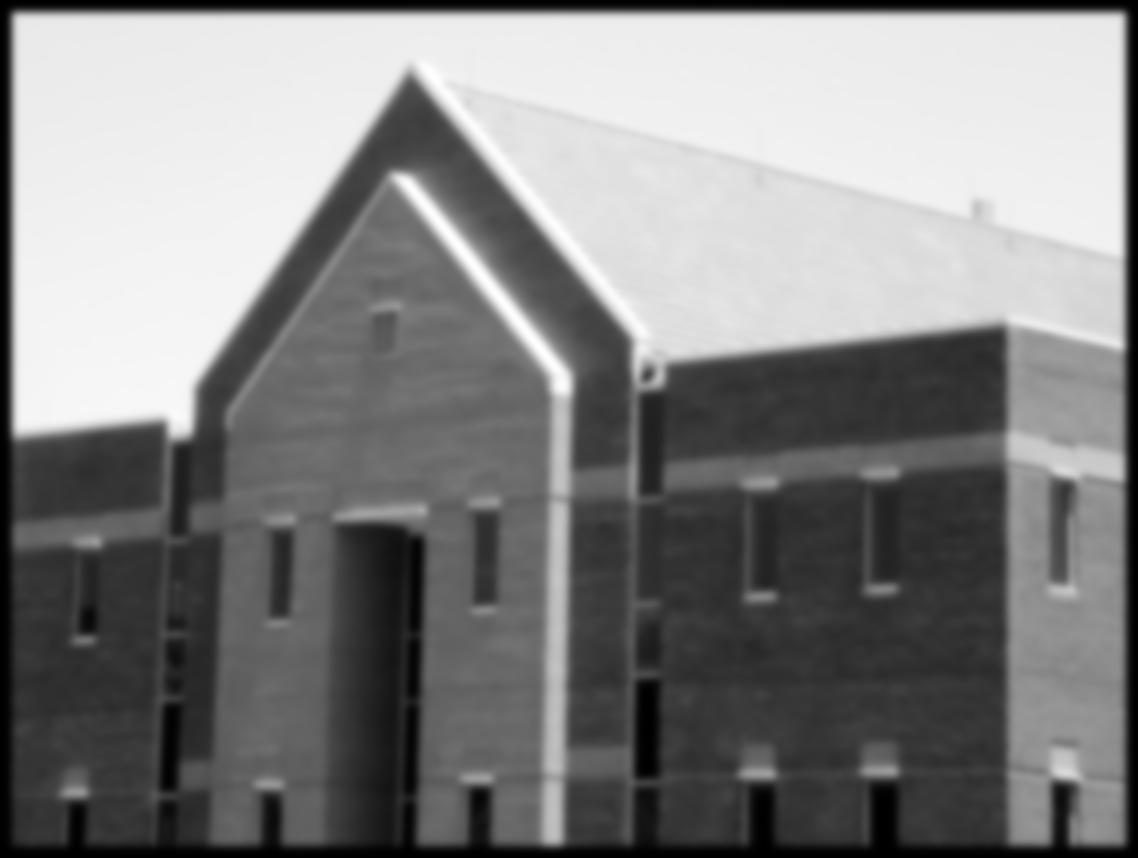
\includegraphics[width=3.5in]{images/im1}
  		\captionof{figure}{$Ig$. Imagem ap\'os convolucao com a gaussiana.}
		\end{minipage}
		

		\begin{minipage}{\linewidth}
  		\centering
  		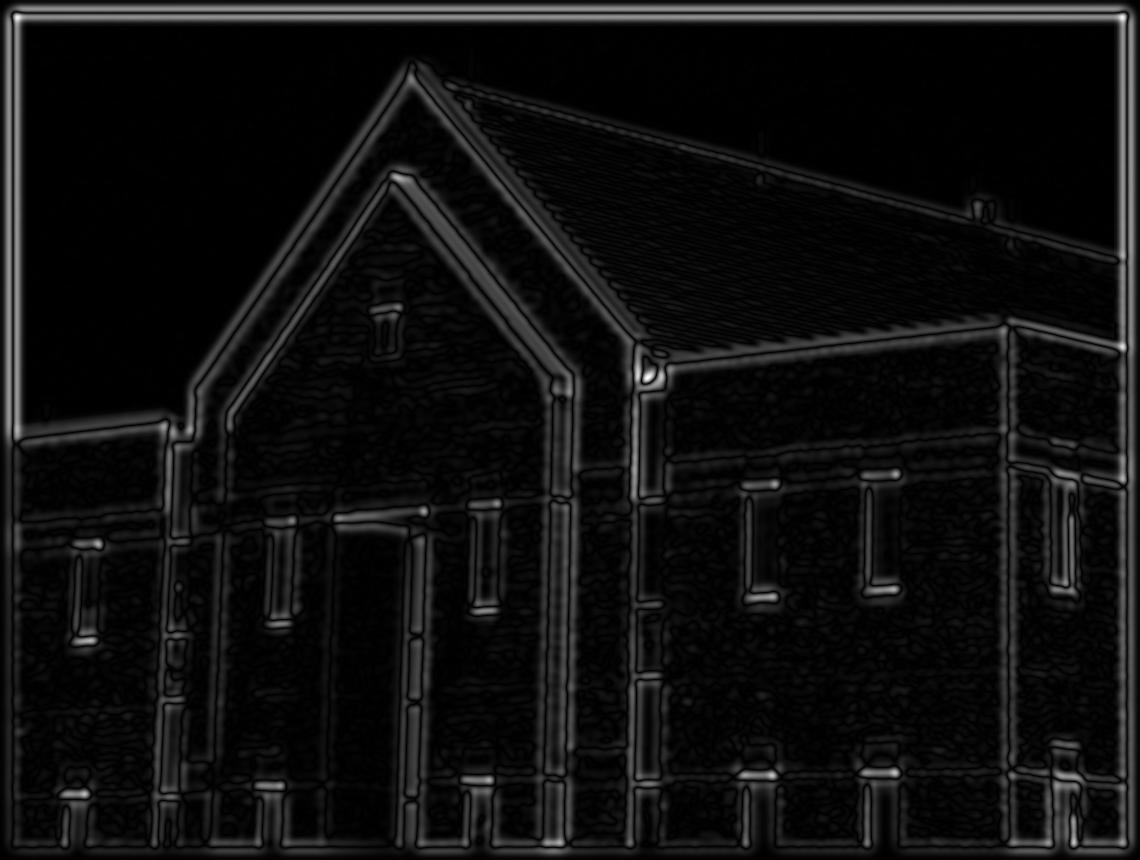
\includegraphics[width=3.5in]{images/im2}
  		\captionof{figure}{$Ilog$. Laplaciano de $Ig$.}
		\end{minipage}
 		

		\begin{minipage}{\linewidth}
  		\centering
  		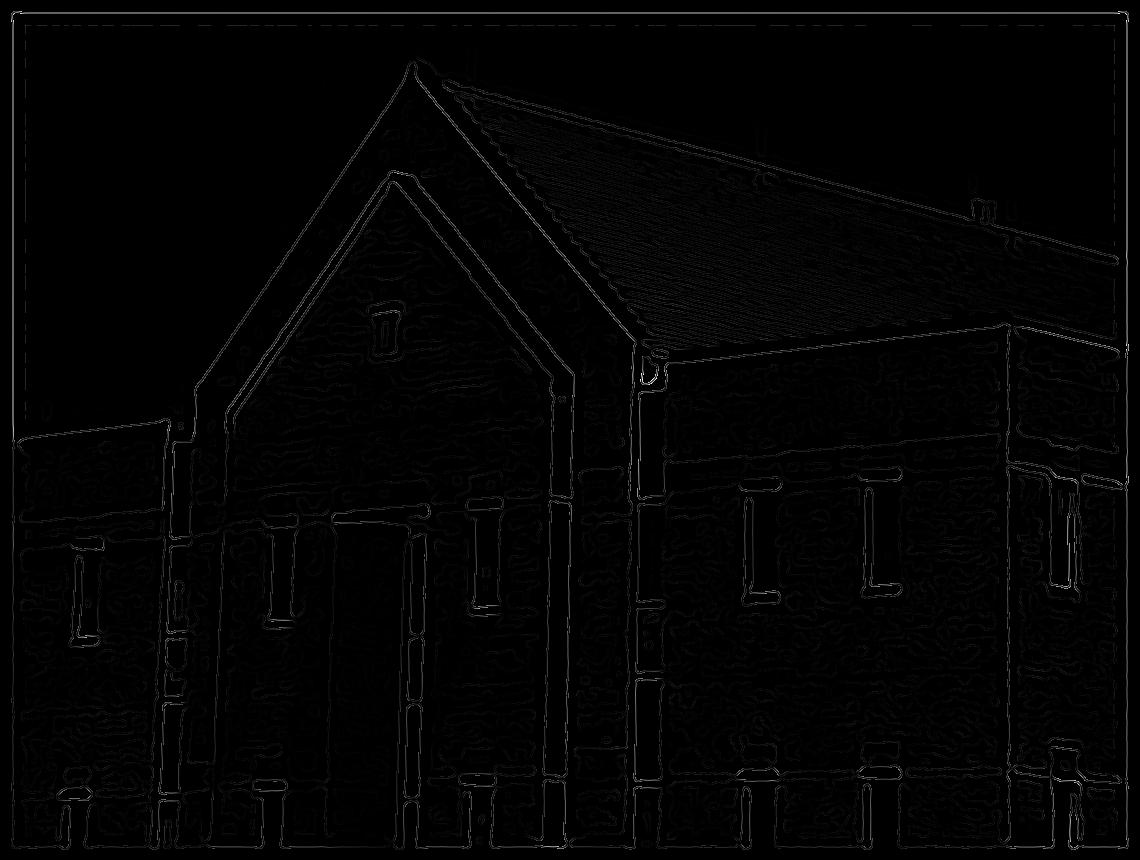
\includegraphics[width=3.5in]{images/im3}
  		\captionof{figure}{$IlogM$. $Ilog$ mascarada pelo cruzamento por zeros. }
		\end{minipage}
 		
 
		\begin{minipage}{\linewidth}
  		\centering
  		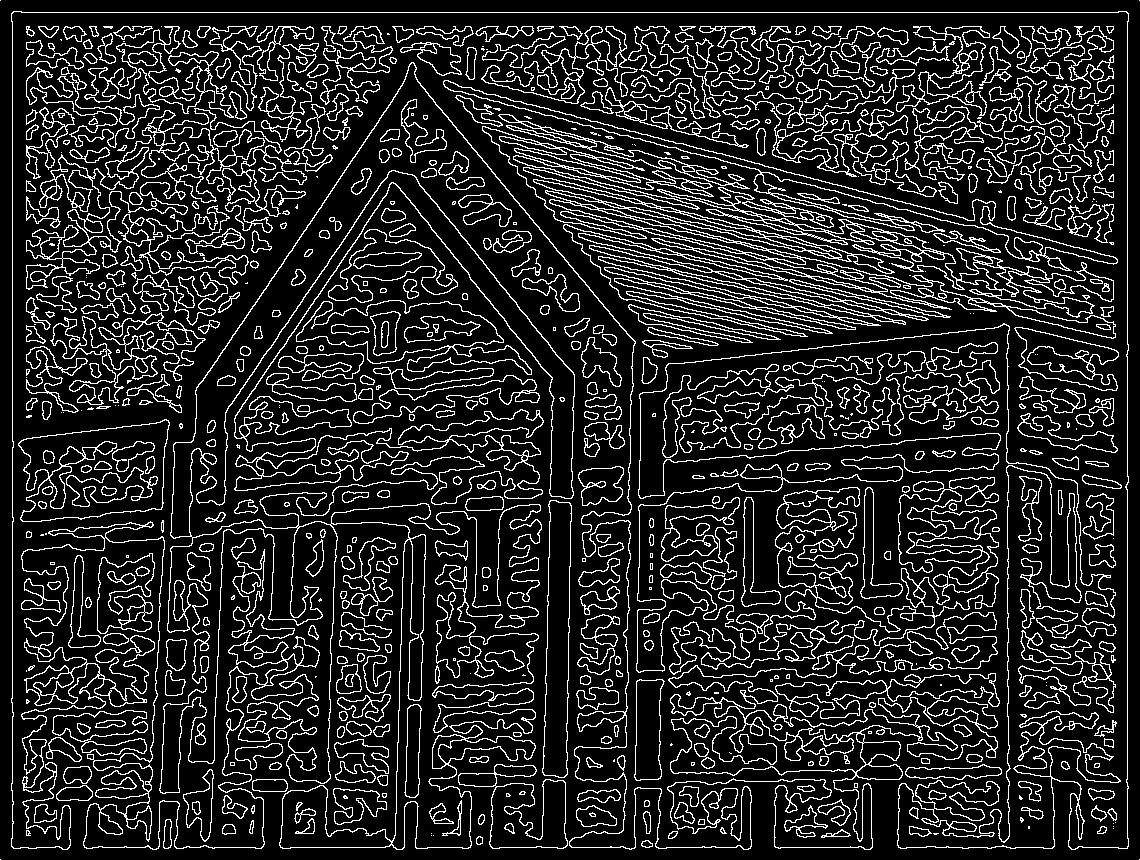
\includegraphics[width=3.5in]{images/im4}
  		\captionof{figure}{$final$. Torna-se bem claro o efeito espaguete.}
		\end{minipage}		
 		

		\begin{minipage}{\linewidth}
  		\centering
  		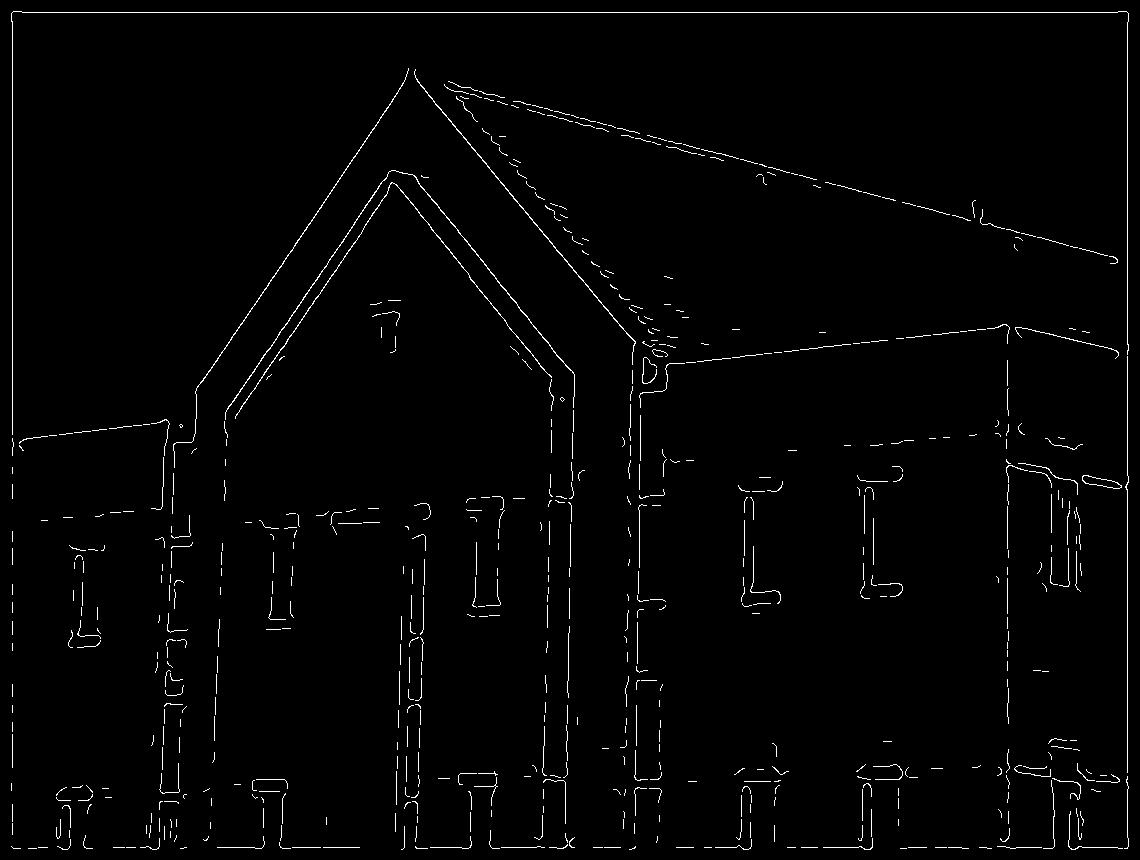
\includegraphics[width=3.5in]{images/im5}
  		\captionof{figure}{$final2$. Resultado apos o limiar e retirada de componentes.}
		\end{minipage}
		 		
	
\section{Conclus\~ao} 
\label{sec:meth} 

Atrav\'es do algoritmo proposto por  Marr-Hildreth pode-se extrair bordas com boa precis\~ao,mas faz-se necess\'ario um p\'os-processamente para retirar o ru\'ido proveniente do efeito espaguete.

\section{Refer\^encias} 
\label{sec:meth} 

[1] R. C. Gonzalez and R. E. Woods, Digital Image Processing,
Prentice-Hall, EUA, 2nd edition, 2002.
\end{document}